1. A partir del archivo \texttt{database-sucia-citi.csv} extraer 
aquellos datos que son relevantes para ser cargados a la tabla 
Branch del repositorio ServiciosFinancieros y guardar el archivo 
'Branch.csv' con campos delimitados por comas con nombre.

\vspace{0.5 cm}

\begin{table}[H]
    \centering
    \resizebox{\textwidth}{!}
    {
        \rowcolors{2}{rowgray}{white}
        \begin{tabular}{llllllllrrrrrrrrr}
            \toprule
            
            \rowcolor{headerblue}
            {
                \color{headertext}\textbf{Institution}
            } &
            {
                \color{headertext}\textbf{Branch Name}
            } &
            {
                \color{headertext}\textbf{Estab. Date}
            } &
            {
                \color{headertext}\textbf{Acq. Date}
            } &
            {
                \color{headertext}\textbf{Street Address}
            } &
            {
                \color{headertext}\textbf{County}
            } &
            {
                \color{headertext}\textbf{State}
            } &
            {
                \color{headertext}\textbf{Zipcode}
            } &
            {
                \color{headertext}\textbf{Latitude}
            } &
            {
                \color{headertext}\textbf{Longitude}
            } &
            {
                \color{headertext}\textbf{2010 Dep}
            } &
            {
                \color{headertext}\textbf{2011 Dep}
            } &
            {
                \color{headertext}\textbf{2012 Dept}
            } &
            {
                \color{headertext}\textbf{2013 Dept}
            } &
            {
                \color{headertext}\textbf{2014 Dept}
            } &
            {
                \color{headertext}\textbf{2015 Dept}
            } &
            {
                \color{headertext}\textbf{2016 Depo}
            } \\
            
            \midrule
            Citi Bank & O boston branch 4 de enero de 2003 & & 08/16/2008 & 50 ROWES WHARF, FLOOR 4 & Suffolk & MA & 2110 & 42.35397 & -71.0498 & 0 & 0 & 0 & 0 & 0 & 0 & 0 \\
            Citi Bank & O milford (ford s/09/16/1957 & & 07/14/1996 & 370 BOSTON POST ROAD & New Haven & CT & 6460 & 41.22554 & -73.0712 & 82623 & 83772 & 86939 & 86705 & 87268 & 89086 & 99210 \\
            Citi Bank & O milford bankin 7 de enero de 2010 & & & 1651 BOSTON POST ROAD & & CT & 6460 & 41.24732 & -73.0252 & & 5102 & 11047 & 18696 & 24017 & 28134 & 33414 \\
            Citi Bank & O monroe ct brar 8 de agosto de 1979 & & 07/14/1996 & 456 MONROE TURNPIKE & Fairfield & CT & 6468 & 41.31428 & -73.2184 & 63203 & 66795 & 68238 & 76666 & 79725 & 82939 & 84911 \\
            Citi Bank & O newtown bran 12/28/1974 & & 07/14/1996 & 30 CHURCH HILL ROAD & Fairfield & CT & 6470 & 41.41458 & -73.3016 & 51729 & 58509 & 65722 & 76224 & 84761 & 87607 & 100543 \\
            Citi Bank & O boston post ro 12 de agosto de 2009 & & & 262 BOSTON POST ROAD & New Haven & CT & 6477 & 41.26741 & -73.0007 & 11091 & 22112 & 35691 & 47681 & 70920 & 76043 & 82218 \\
            Citi Bank & O shelton branch 7 de octubre de 1982 & & 07/14/1996 & 675 BRIDGEPORT AVENUE & Fairfield & CT & 6484 & 41.27746 & -73.1215 & 67941 & 62727 & 65088 & 70702 & 85390 & 82766 & 93207 \\
            Citi Bank & O southbury grec 11 de julio de 2011 & & & 775 MAIN STREET SOUTH & New Haven & CT & 6488 & 41.46931 & -73.2346 & & 6638 & 16492 & 27050 & 35887 & 45501 & \\
            \bottomrule
        \end{tabular}
    }
    \caption{Tabla fea de la práctica.}
    \label{table:1}
\end{table}

\vspace{0.5 cm}

Primero pasaremos el archivo \texttt{database-sucia-citi.csv} 
a DataFrame, esto para poder visualizar las columnas sus datos, 
y en base a estos (porque los encabezados no nos dicen mucho), 
pasar la información al formato de la tabla Branch.

\vspace{1.5 cm}

Recordemos que la tabla \texttt{Branch} tiene la siguiente estructura:

\begin{table}[H]
    \centering
    \resizebox{\textwidth}{!}
    {
        \rowcolors{2}{rowgray}{white}
        \begin{tabular}{cllccc}
            \toprule
            
            \rowcolor{headerblue}
            {
                \color{headertext}\textbf{branch\_key}
            } &
            {
                \color{headertext}\textbf{branch\_name}
            } &
            {
                \color{headertext}\textbf{branch\_address}
            } &
            {
                \color{headertext}\textbf{branch\_city}
            } &
            {
                \color{headertext}\textbf{branch\_state}
            } &
            {
                \color{headertext}\textbf{branch\_zip}
            } \\
            
            \midrule
            1 & Big Apple  & 822 Financial Way  & New York     & NY & 46842 \\
            2 & Philly     & 15 Financial Way   & Philadelphia & PA & 36769 \\
            3 & Windy City & 923 Financial Way  & Chicago      & IL & 43389 \\
            4 & Tinseltown & 945 Financial Way  & Los Angeles  & CA & 80626 \\
            \bottomrule
        \end{tabular}
    }
    \caption{Estructura de la tabla \texttt{Branch}.}
    \label{table:2}
\end{table}

Nota: en esta tabla ignoramos el \texttt{branch\_type} porque no encontramos un 
equivalente en el archivo csv (y porque no viene en la tabla de la práctica), 
pero lo agregaremos en una columna sin contenido.

\vspace{0.5 cm}

Usamos \texttt{Python} para hacer la extracción de los datos del archivo csv, 
pues es lo que mejor sabemos usar. 

Los pasos a seguir para el \texttt{script1} fueron:

\begin{enumerate}
    \item Importar las bibliotecas necesarias 
    \item Leer el archivo \texttt{database-sucia-citi.csv} 
    \item Convertir el archivo original a DataFrame
    \item Renombrar las columnas que tienen la información solicitada.
    \item Hacer una copia del DataFrame, para no modificar el original.
    \item Crear las columas que nos hagan falta y no tengan un equivalente.
    \item Llenar las columnas creadas con la información que sea necesaria. 
    \item Ordenar las columnas conforme a los requerimientos.
    \item Pasar el DataFrame a \texttt{csv} y guardarlo.
    \item Comprobar los cambios realizados.
\end{enumerate} 

\vspace{0.5 cm}

\lstinputlisting[
    language = Python,
    caption = {Extracción de datos.},
    label = {lst:script1}
]{D:/IIMAS/Base de datos/P4 - DWH - Extraccion y perfilado/script1.py}

\vspace{0.5 cm}

\subsection*{Resultados}

\begin{figure}[H]
    \centering
    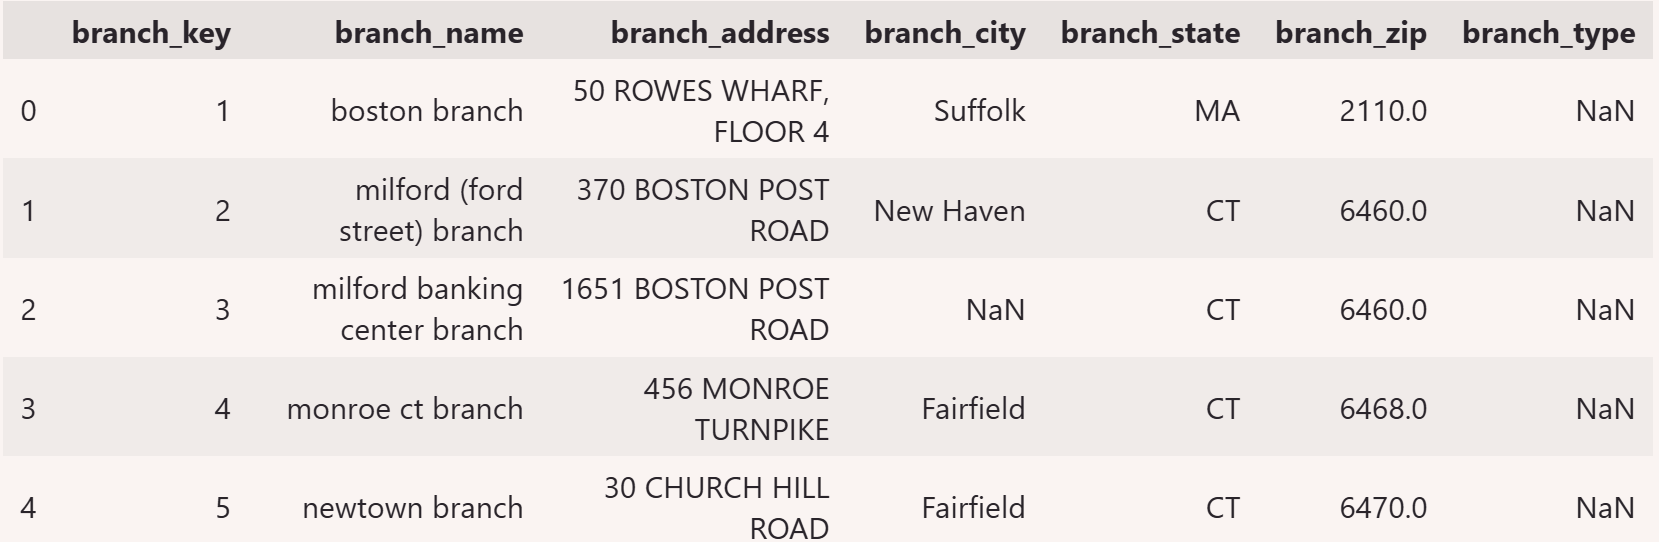
\includegraphics[width = 1\textwidth]{TablaBranch.png}
    \caption{Tabla \texttt{Branch.csv} (vista desde Jupyter Notebook).}
    \label{fig:TB}
\end{figure}

\newpage